% Created 2014-10-11 sáb 16:39
\documentclass[xcolor={usenames,svgnames,dvipsnames}]{beamer}
\usepackage[utf8]{inputenc}
\usepackage[T1]{fontenc}
\usepackage{fixltx2e}
\usepackage{graphicx}
\usepackage{longtable}
\usepackage{float}
\usepackage{wrapfig}
\usepackage{rotating}
\usepackage[normalem]{ulem}
\usepackage{amsmath}
\usepackage{textcomp}
\usepackage{marvosym}
\usepackage{wasysym}
\usepackage{amssymb}
\usepackage{hyperref}
\tolerance=1000
\usepackage{color}
\usepackage{listings}
\AtBeginSection[]{\begin{frame}[plain]\tableofcontents[currentsection,hideallsubsections]\end{frame}}
\lstset{keywordstyle=\color{blue}, commentstyle=\color{gray!90}, basicstyle=\ttfamily\small, columns=fullflexible, breaklines=true,linewidth=\textwidth, backgroundcolor=\color{gray!23}, basewidth={0.5em,0.4em}, literate={á}{{\'a}}1 {ñ}{{\~n}}1 {é}{{\'e}}1 {ó}{{\'o}}1 {º}{{\textordmasculine}}1}
\usepackage{mathpazo}
\hypersetup{colorlinks=true, linkcolor=Blue, urlcolor=Blue}
\usepackage{fancyvrb}
\DefineVerbatimEnvironment{verbatim}{Verbatim}{boxwidth=\textwidth, fontsize=\tiny, formatcom = {\color{black!70}}}
\usepackage{animate}
\usetheme{Goettingen}
\usecolortheme{rose}
\usefonttheme{serif}
\author{Oscar Perpiñán Lamigueiro}
\date{24 de Octubre de 2014}
\title{Visualización de datos raster}
\hypersetup{
  pdfkeywords={},
  pdfsubject={},
  pdfcreator={Emacs 24.3.1 (Org mode 8.2.7c)}}
\begin{document}

\maketitle

\section{Introducción}
\label{sec-1}

\begin{frame}[label=sec-1-1]{Datos raster}
\end{frame}
\begin{frame}[fragile,label=sec-1-2]{Paquete raster}
 \begin{itemize}
\item Define funciones para crear, leer, manipular y escribir datos raster.
\item Implementa algebra raster y funciones de uso común en GIS.
\item Es capaz de trabajar con ficheros muy grandes trabajando en disco y procesando por lotes.
\item Clases:
\begin{itemize}
\item \texttt{RasterLayer}
\item \texttt{RasterBrick}
\item \texttt{RasterStack}
\end{itemize}
\end{itemize}
\end{frame}

\begin{frame}[fragile,label=sec-1-3]{Paquete raster}
 \begin{itemize}
\item Funciones básicas: \texttt{abs}, \texttt{round}, \texttt{ceiling}, \texttt{floor}, \texttt{trunc},
\texttt{sqrt}, \texttt{log}, \texttt{log10}, \texttt{exp}, \texttt{cos}, \texttt{sin}, \texttt{max}, \texttt{min}, \texttt{range},
\texttt{prod}, \texttt{sum}, \texttt{any}, \texttt{all}.
\item Se pueden mezclar objetos \texttt{Raster*} con números.
\end{itemize}
\end{frame}

\begin{frame}[fragile,label=sec-1-4]{Funciones para modificar contenido y extensión, o para combinar objetos:}
 \begin{itemize}
\item The \texttt{crop} function takes a geographic subset of a larger
\texttt{Raster*} object. \texttt{trim} crops a \texttt{RasterLayer}
by removing the outer rows and columns that only contain \texttt{NA}
values. \texttt{extend} adds new rows and/or columns with
\texttt{NA} values.
\item The \texttt{merge} function merges two or more \texttt{Raster*}
    objects into a single new object.
\item \texttt{projectRaster} transforms values of a \texttt{Raster*}
    object to a new object with a different coordinate reference system.
\end{itemize}
\end{frame}
\begin{frame}[fragile,label=sec-1-5]{Funciones para modificar contenido y extensión, o para combinar objetos:}
 \begin{itemize}
\item With \texttt{overlay}, multiple \texttt{Raster*} objects can be
combined (for example, multiply them).
\item \texttt{mask} removes all values from one layer that are
\texttt{NA} in another layer, and \texttt{cover} combines two layers
by taking the values of the first layer except where these are
\texttt{NA}.
\end{itemize}
\end{frame}
\begin{frame}[fragile,label=sec-1-6]{Funciones para modificar contenido y extensión, o para combinar objetos:}
 \begin{itemize}
\item \texttt{calc} computes a function for a \texttt{Raster*}
object. With \texttt{RasterLayer} objects, another
\texttt{RasterLayer} is returned. With multilayer objects the result
depends on the function: With a summary function (\texttt{sum},
\texttt{max}, etc.),  \texttt{calc} returns a \texttt{RasterLayer}
object, and a \texttt{RasterBrick} object otherwise.
\item \texttt{stackApply} computes summary layers for subsets of a
\texttt{RasterStack} or \texttt{RasterBrick}.
\end{itemize}
\end{frame}
\begin{frame}[fragile,label=sec-1-7]{Funciones para modificar contenido y extensión, o para combinar objetos:}
 \begin{itemize}
\item \texttt{cut} and \texttt{reclassify} replace ranges of values
with single values.
\item \texttt{zonal} computes zonal statistics, that is, summarizes a
\texttt{Raster*} object using zones (areas with the same integer
number) defined by another \texttt{RasterLayer}.
\end{itemize}
\end{frame}

\begin{frame}[fragile,label=sec-1-8]{Paquete \texttt{rasterVis}}
\end{frame}

\section{Datos Cuantitativos}
\label{sec-2}

\begin{frame}[fragile,label=sec-2-1]{Datos}
 \lstset{language=R,label= ,caption= ,numbers=none}
\begin{lstlisting}
  library(raster)
  library(rasterVis)
  SISav <- raster('data/SISav')
  levelplot(SISav)
\end{lstlisting}
\end{frame}

\begin{frame}[label=sec-2-2]{}
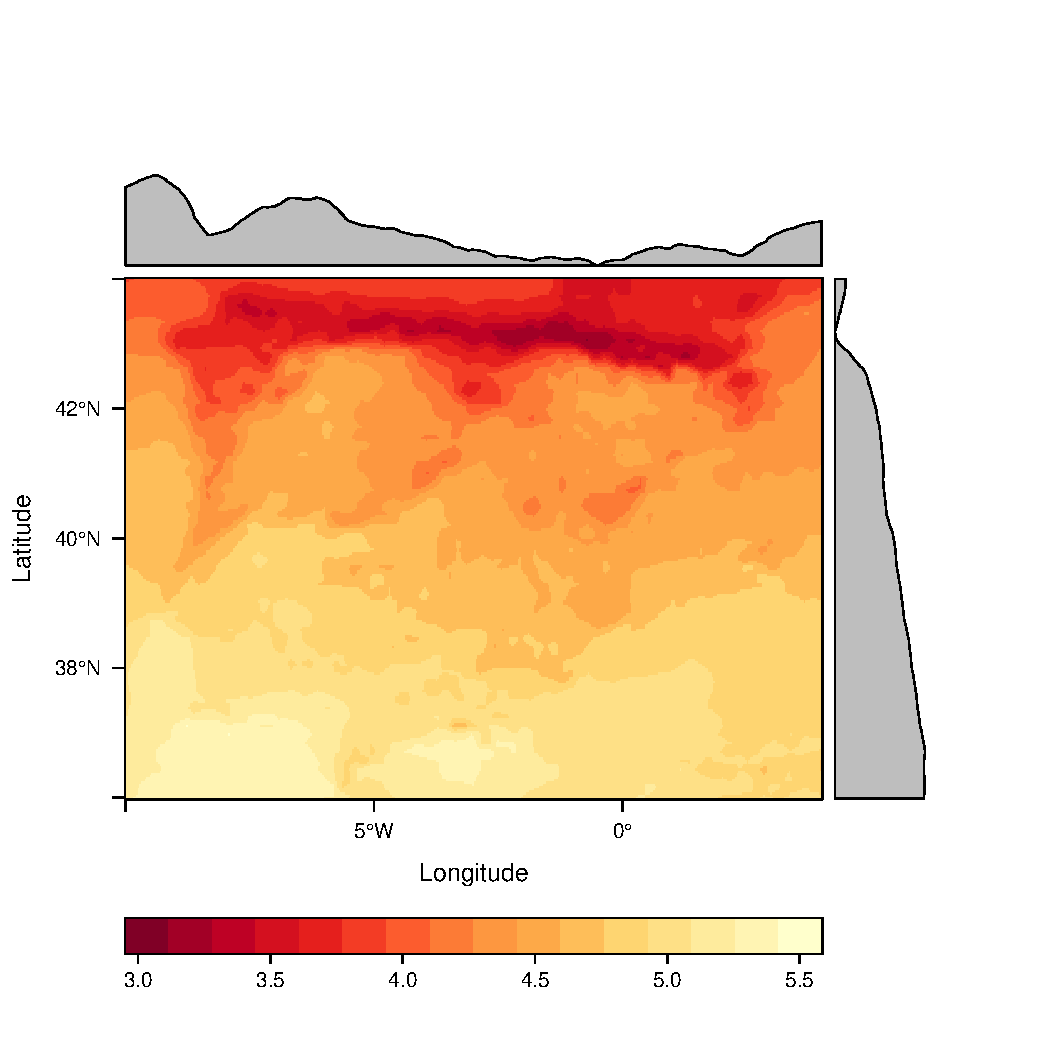
\includegraphics[width=.9\linewidth]{figs/leveplotSISavOrig.pdf}
\end{frame}

\begin{frame}[fragile,label=sec-2-3]{Fronteras}
 \lstset{language=R,label= ,caption= ,numbers=none}
\begin{lstlisting}
  library(maps)
  library(mapdata)
  library(maptools)
  
  ext <- as.vector(extent(SISav))
  boundaries <- map('worldHires',
                    xlim=ext[1:2], ylim=ext[3:4],
                    plot=FALSE)
  boundaries <- map2SpatialLines(boundaries,
                                 proj4string=CRS(projection(SISav)))
\end{lstlisting}
\end{frame}

\begin{frame}[fragile,label=sec-2-4]{Fronteras}
 \lstset{language=R,label= ,caption= ,numbers=none}
\begin{lstlisting}
  levelplot(SISav) + layer(sp.lines(boundaries, lwd=0.5))
\end{lstlisting}

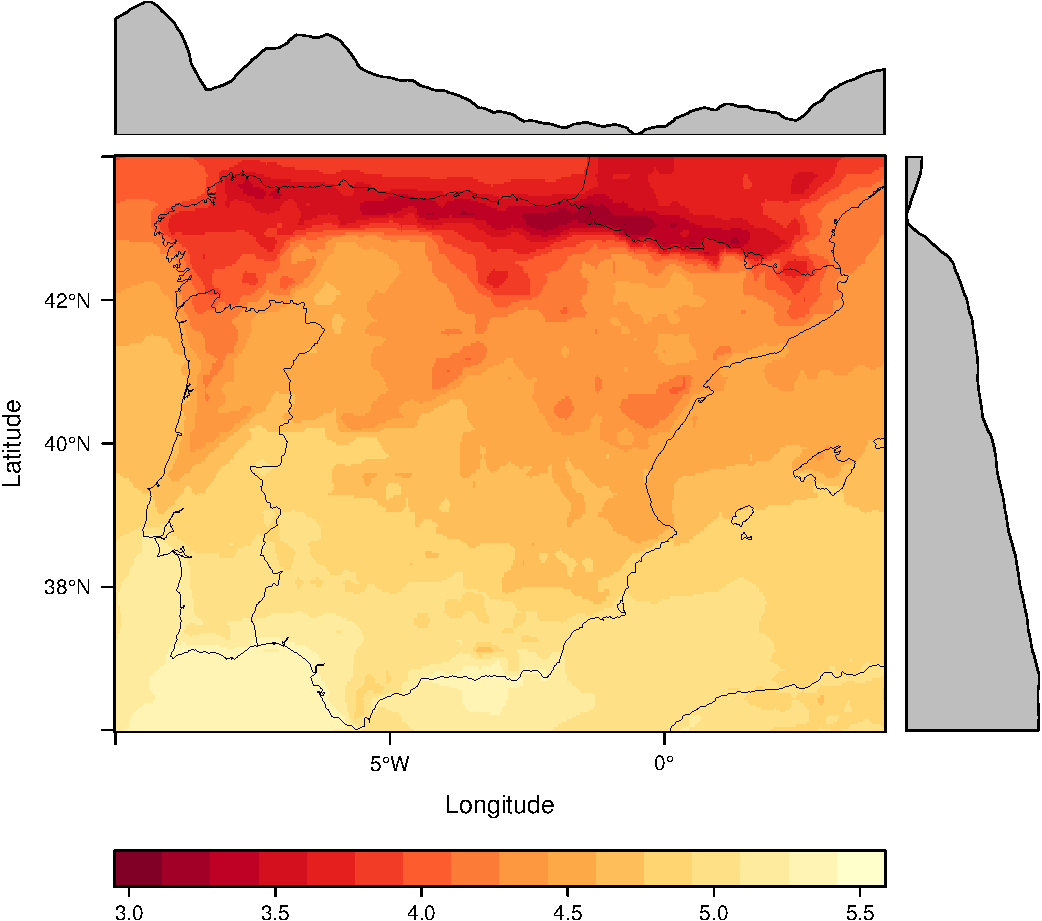
\includegraphics[width=.9\linewidth]{figs/leveplotSISavBoundaries.pdf}
\end{frame}

\begin{frame}[fragile,label=sec-2-5]{Hill shading}
 \begin{itemize}
\item Download a Digital Elevation Model (DEM) from the DIVA-GIS service.
\end{itemize}

\lstset{language=R,label= ,caption= ,numbers=none}
\begin{lstlisting}
  old <- setwd(tempdir())
  download.file('http://biogeo.ucdavis.edu/data/diva/msk_alt/ESP_msk_alt.zip, 'ESP_msk_alt.zip')
  unzip('ESP_msk_alt.zip', exdir='.')
  
  DEM <- raster('ESP_msk_alt')
\end{lstlisting}
\end{frame}

\begin{frame}[fragile,label=sec-2-6]{Hill shading}
 \begin{itemize}
\item Compute the hill shade raster with \texttt{terrain} and \texttt{hillShade} from \texttt{raster}.
\end{itemize}

\lstset{language=R,label= ,caption= ,numbers=none}
\begin{lstlisting}
  slope <- terrain(DEM, 'slope')
  aspect <- terrain(DEM, 'aspect')
  hs <- hillShade(slope=slope, aspect=aspect,
                  angle=20, direction=30)
\end{lstlisting}

\lstset{language=R,label= ,caption= ,numbers=none}
\begin{lstlisting}
  setwd(old)
\end{lstlisting}
\end{frame}

\begin{frame}[fragile,label=sec-2-7]{Hill Shading}
 \begin{itemize}
\item Combine the result with the previous map using semitransparency.
\end{itemize}

\lstset{language=R,label= ,caption= ,numbers=none}
\begin{lstlisting}
  ## hillShade theme: gray colors and semitransparency
  hsTheme <- modifyList(GrTheme(), list(regions=list(alpha=0.6)))
  
  levelplot(SISav, panel=panel.levelplot.raster,
            margin=FALSE, colorkey=FALSE) +
      levelplot(hs, par.settings=hsTheme, maxpixels=1e6) +
      layer(sp.lines(boundaries, lwd=0.5))
\end{lstlisting}
\end{frame}

\begin{frame}[label=sec-2-8]{}
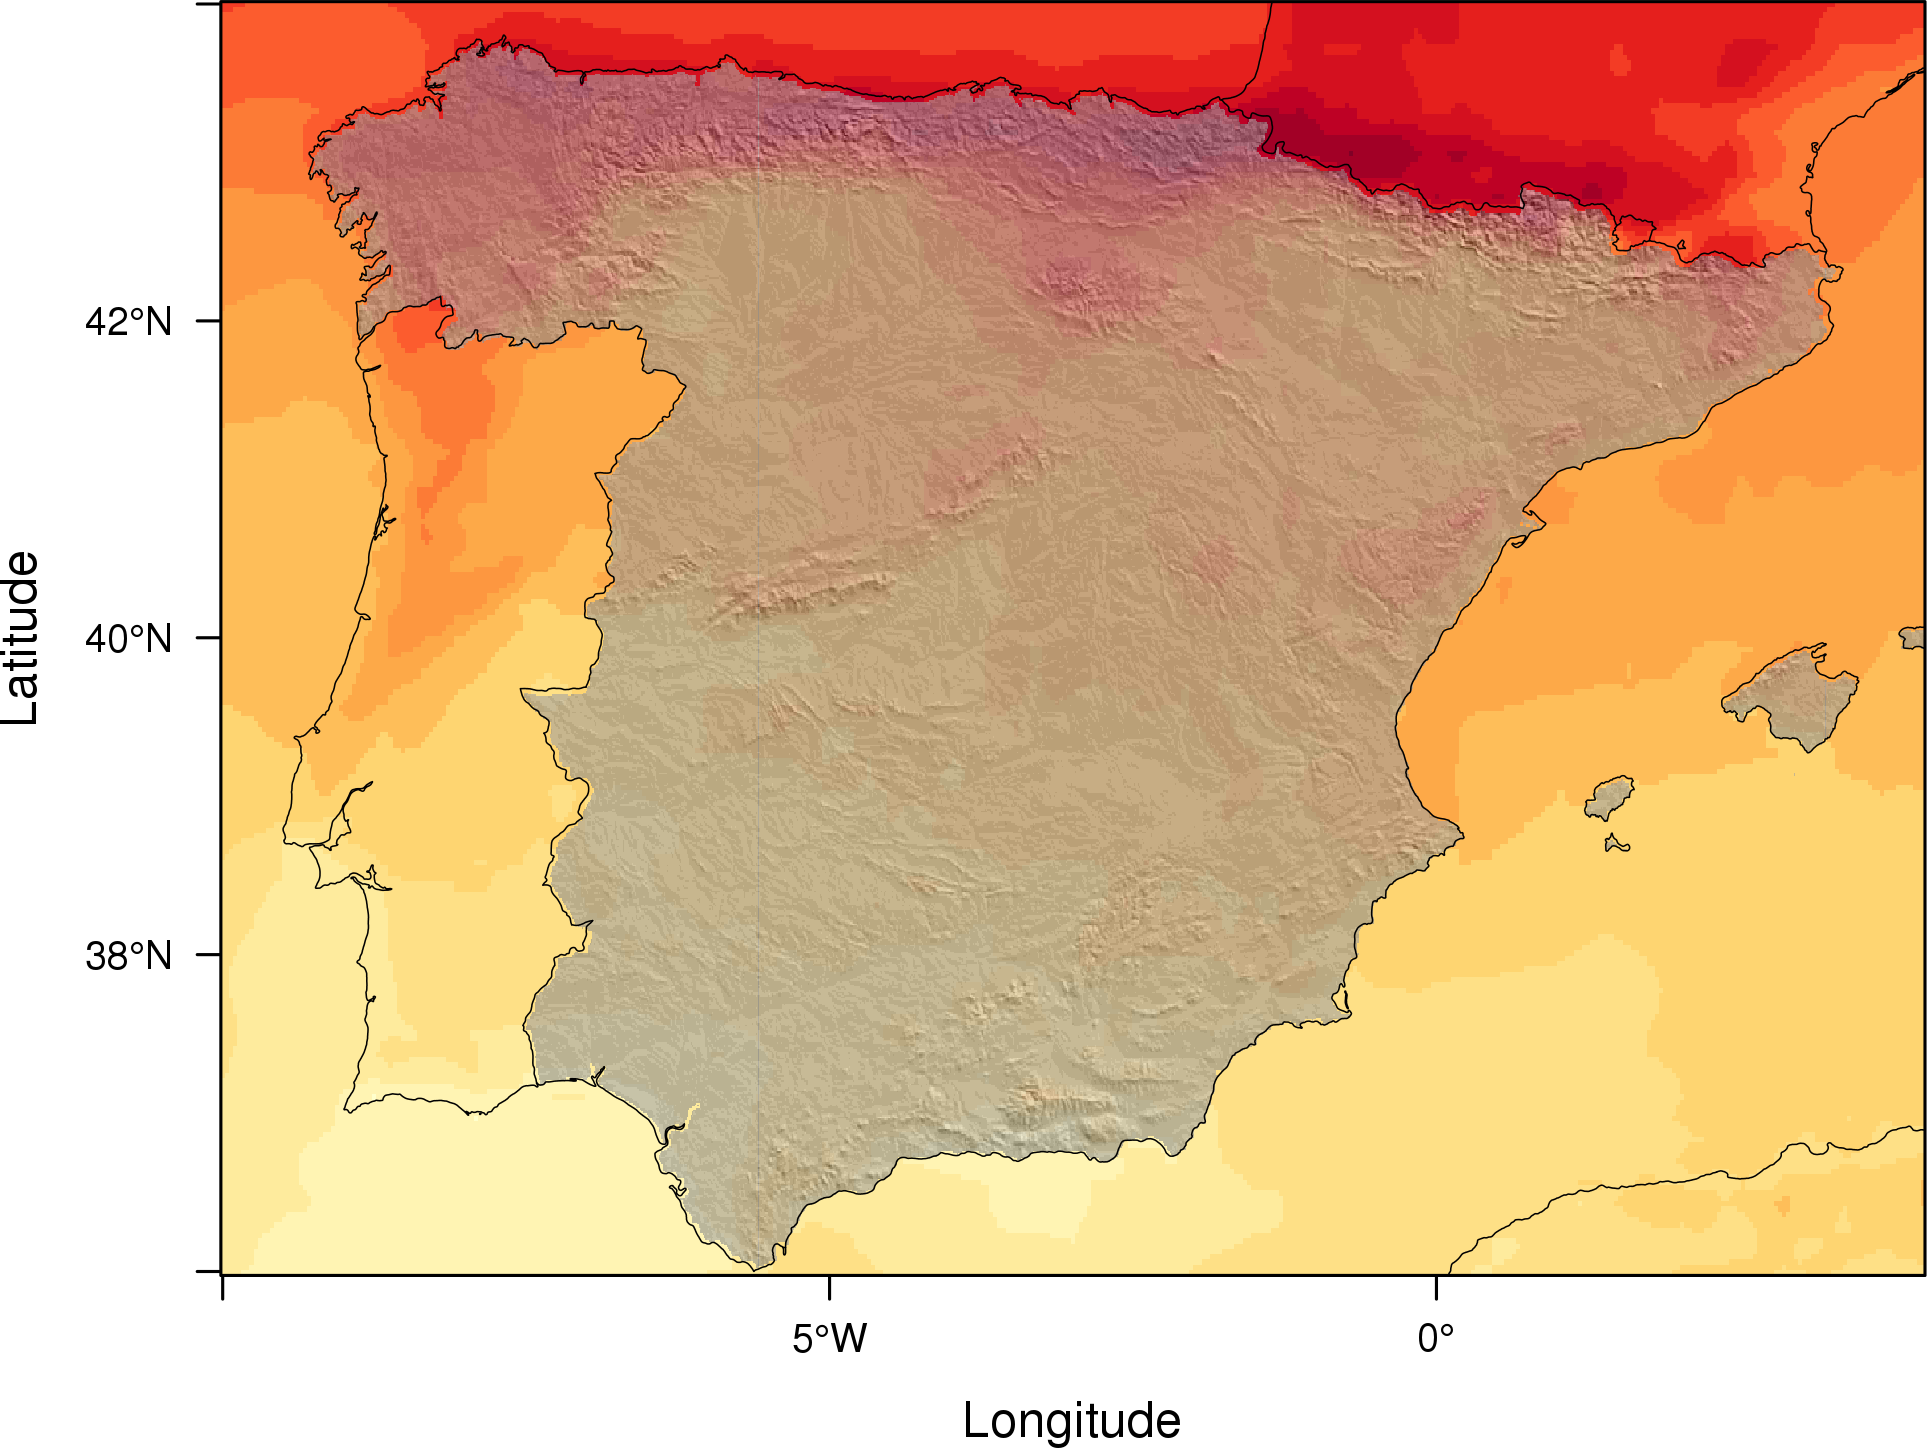
\includegraphics[width=.9\linewidth]{figs/hillShading.png}
\end{frame}

\begin{frame}[fragile,label=sec-2-9]{3D}
 \lstset{language=R,label= ,caption= ,numbers=none}
\begin{lstlisting}
  plot3D(DEM, maxpixels=5e4)
\end{lstlisting}

The output scene can be exported to several formats such as WebGL with
\texttt{writeWebGL} to be rendered in a browser, or \texttt{STL} with \texttt{writeSTL}, a
format commonly used in 3D printing. Files using this format are
\href{https://github.com/oscarperpinan/spacetime-vis/blob/gh-pages/images/DEM.stl}{viewed easily on GitHub}.

\lstset{language=R,label= ,caption= ,numbers=none}
\begin{lstlisting}
writeSTL('figs/DEM.stl')
\end{lstlisting}
\end{frame}

\section{Datos Categóricos}
\label{sec-3}
\begin{frame}[fragile,label=sec-3-1]{Datos}
 This section illustrates how to read and display rasters with
categorical information using information from the NEO-NASA
project. 
\lstset{language=R,label= ,caption= ,numbers=none}
\begin{lstlisting}
  library(raster)
  ## China and India  
  ext <- extent(65, 135, 5, 55)
  
  pop <- raster('data/875430rgb-167772161.0.FLOAT.TIFF')
  pop <- crop(pop, ext)
  pop[pop==99999] <- NA
  
  landClass <- raster('data/241243rgb-167772161.0.TIFF')
  landClass <- crop(landClass, ext)
\end{lstlisting}
\end{frame}

\begin{frame}[fragile,label=sec-3-2]{RAT}
 \lstset{language=R,label= ,caption= ,numbers=none}
\begin{lstlisting}
  landClass[landClass %in% c(0, 254)] <- NA
  ## Only four groups are needed:
  ## Forests: 1:5
  ## Shrublands, etc: 6:11
  ## Agricultural/Urban: 12:14
  ## Snow: 15:16
  landClass <- cut(landClass, c(0, 5, 11, 14, 16))
  ## Add a Raster Attribute Table and define the raster as categorical data
  landClass <- ratify(landClass)
  ## Configure the RAT: first create a RAT data.frame using the
  ## levels method; second, set the values for each class (to be
  ## used by levelplot); third, assign this RAT to the raster
  ## using again levels
  rat <- levels(landClass)[[1]]
  rat$classes <- c('Forest', 'Land', 'Urban', 'Snow')
  levels(landClass) <- rat
\end{lstlisting}
\end{frame}

\begin{frame}[fragile,label=sec-3-3]{levelplot}
 \lstset{language=R,label= ,caption= ,numbers=none}
\begin{lstlisting}
  library(rasterVis)
  
  pal <- c('palegreen4', # Forest
           'lightgoldenrod', # Land
           'indianred4', # Urban
           'snow3')      # Snow
  
  catTheme <- modifyList(rasterTheme(),
                         list(panel.background = list(col='lightskyblue1'),
                              regions = list(col= pal)))
  
  levelplot(landClass, maxpixels=3.5e5, par.settings=catTheme,
            panel=panel.levelplot.raster)
\end{lstlisting}
\end{frame}

\begin{frame}[label=sec-3-4]{}
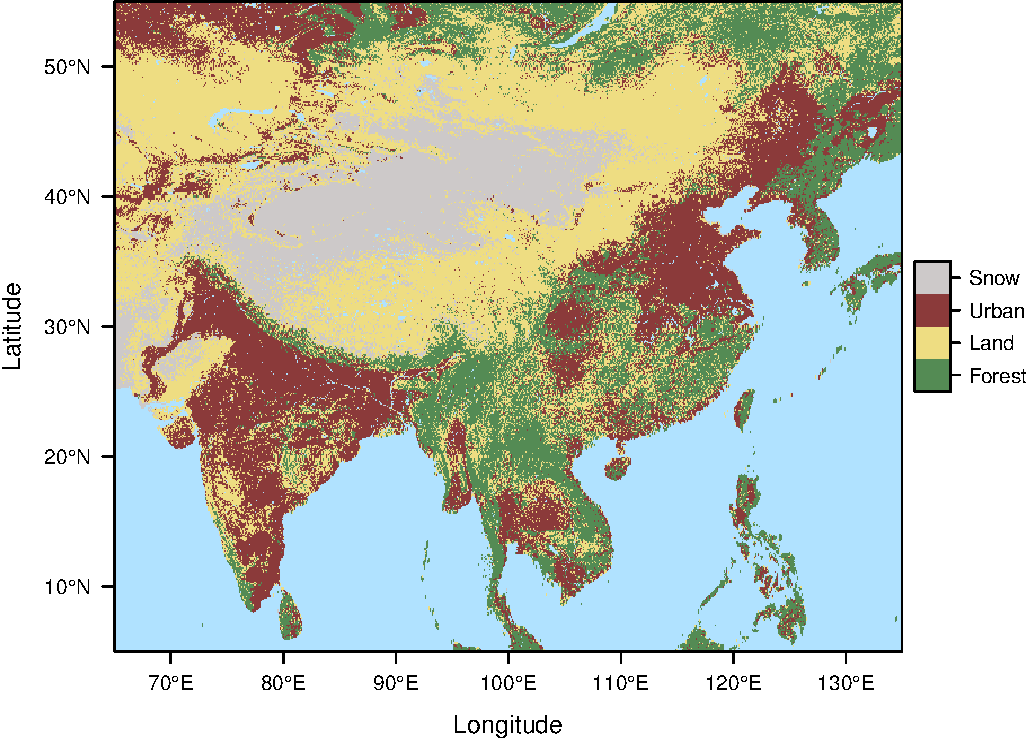
\includegraphics[width=.9\linewidth]{figs/landClass.pdf}
\end{frame}

\begin{frame}[fragile,label=sec-3-5]{Relación con cuantitativos}
 \lstset{language=R,label= ,caption= ,numbers=none}
\begin{lstlisting}
  pPop <- levelplot(pop, zscaleLog=10, par.settings=BTCTheme,
                    maxpixels=3.5e5, panel=panel.levelplot.raster)
  pPop
\end{lstlisting}
\end{frame}

\begin{frame}[label=sec-3-6]{}
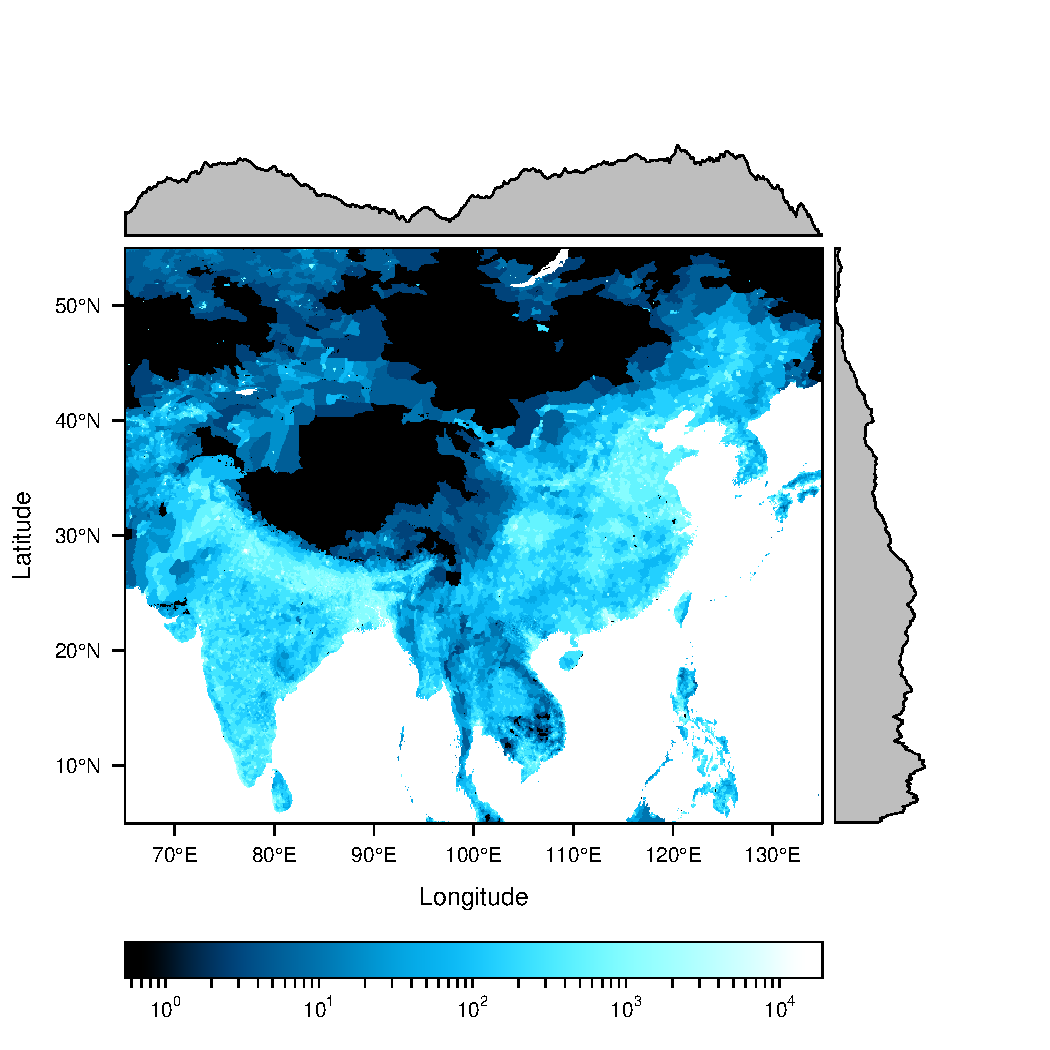
\includegraphics[width=.9\linewidth]{figs/populationNASA.pdf}
\end{frame}

\begin{frame}[fragile,label=sec-3-7]{Histograma}
 \lstset{language=R,label= ,caption= ,numbers=none}
\begin{lstlisting}
  s <- stack(pop, landClass)
  names(s) <- c('pop', 'landClass')
  histogram(~log10(pop)|landClass, data=s,
            scales=list(relation='free'))
\end{lstlisting}

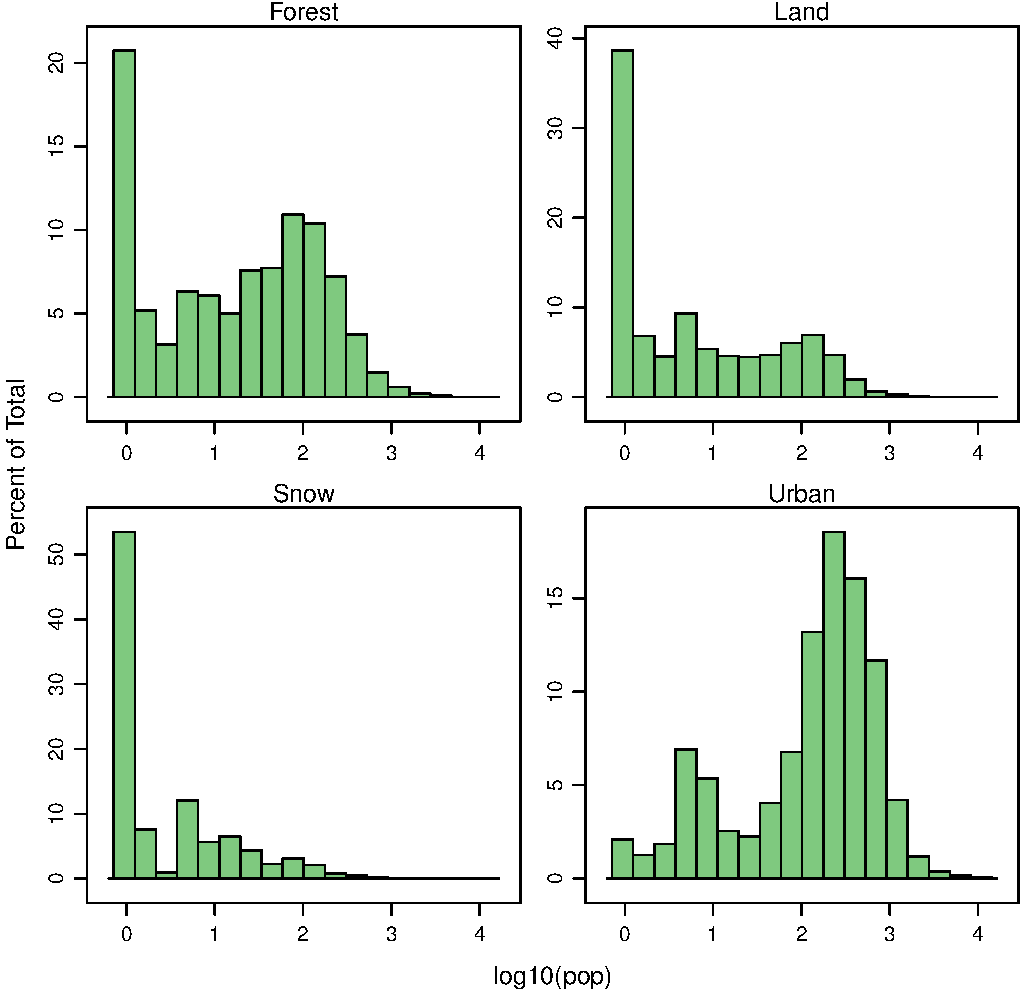
\includegraphics[width=.9\linewidth]{figs/histogramLandClass.pdf}
\end{frame}


\section{Raster Espacio-Temporales}
\label{sec-4}
\begin{frame}[label=sec-4-1]{Introducción}
\end{frame}

\begin{frame}[fragile,label=sec-4-2]{Datos}
 \lstset{language=R,label= ,caption= ,numbers=none}
\begin{lstlisting}
  library(raster)
  library(zoo)
  library(rasterVis)
  
  SISdm <- brick('data/SISgal')
  
  timeIndex <- seq(as.Date('2011-01-01'), by='day', length=365)
  SISdm <- setZ(SISdm, timeIndex)
  names(SISdm) <- format(timeIndex, '%a_%Y%m%d')
\end{lstlisting}
\end{frame}


\begin{frame}[fragile,label=sec-4-3]{Level Plots}
 \lstset{language=R,label= ,caption= ,numbers=none}
\begin{lstlisting}
  levelplot(SISdm, layers=1:12, panel=panel.levelplot.raster)
\end{lstlisting}


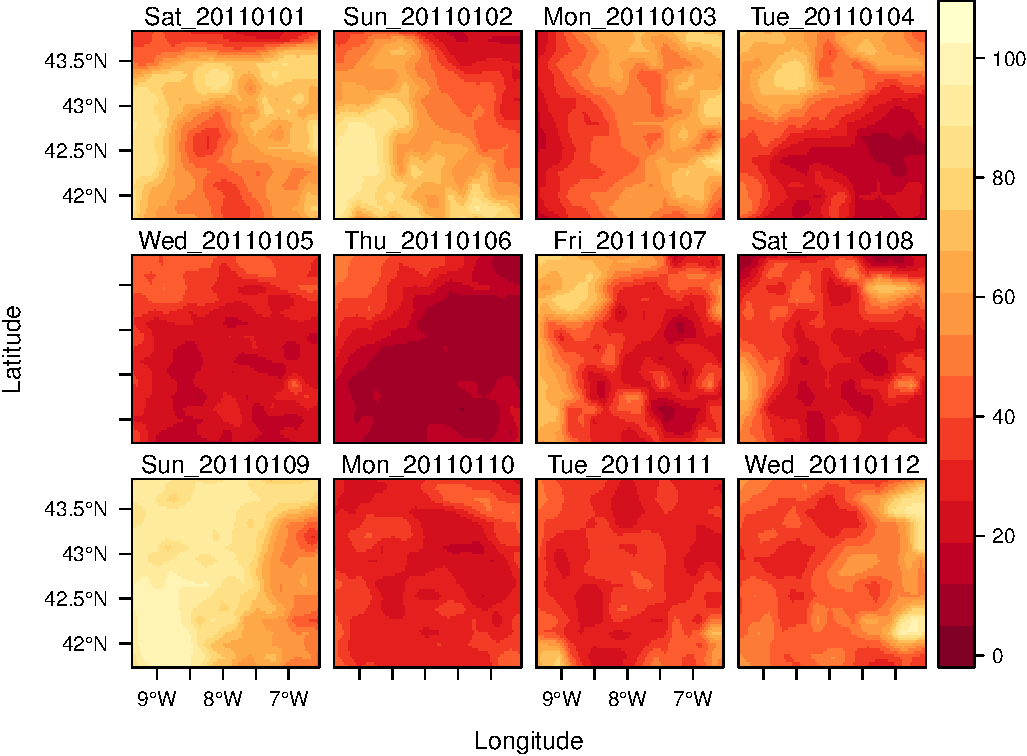
\includegraphics[width=.9\linewidth]{figs/SISdm.pdf}
\end{frame}

\begin{frame}[fragile,label=sec-4-4]{zApply}
 \lstset{language=R,label= ,caption= ,numbers=none}
\begin{lstlisting}
  SISmm <- zApply(SISdm, by=as.yearmon, fun='mean')
\end{lstlisting}
\end{frame}

\begin{frame}[fragile,label=sec-4-5]{}
 \lstset{language=R,label= ,caption= ,numbers=none}
\begin{lstlisting}
  levelplot(SISmm, panel=panel.levelplot.raster)
\end{lstlisting}

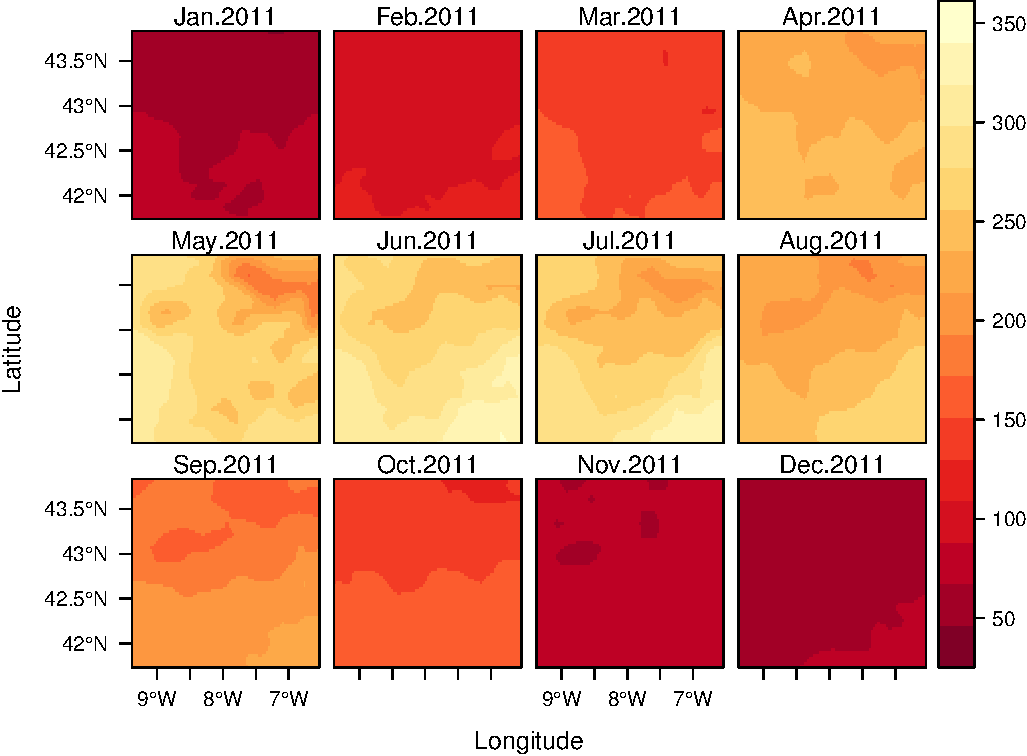
\includegraphics[width=.9\linewidth]{figs/SISmm.pdf}
\end{frame}

\begin{frame}[label=sec-4-6]{Graphical Exploratory Data Analysis}
\end{frame}


\begin{frame}[fragile,label=sec-4-7]{Histogram}
 \lstset{language=R,label= ,caption= ,numbers=none}
\begin{lstlisting}
  histogram(SISdm, FUN=as.yearmon)
\end{lstlisting}

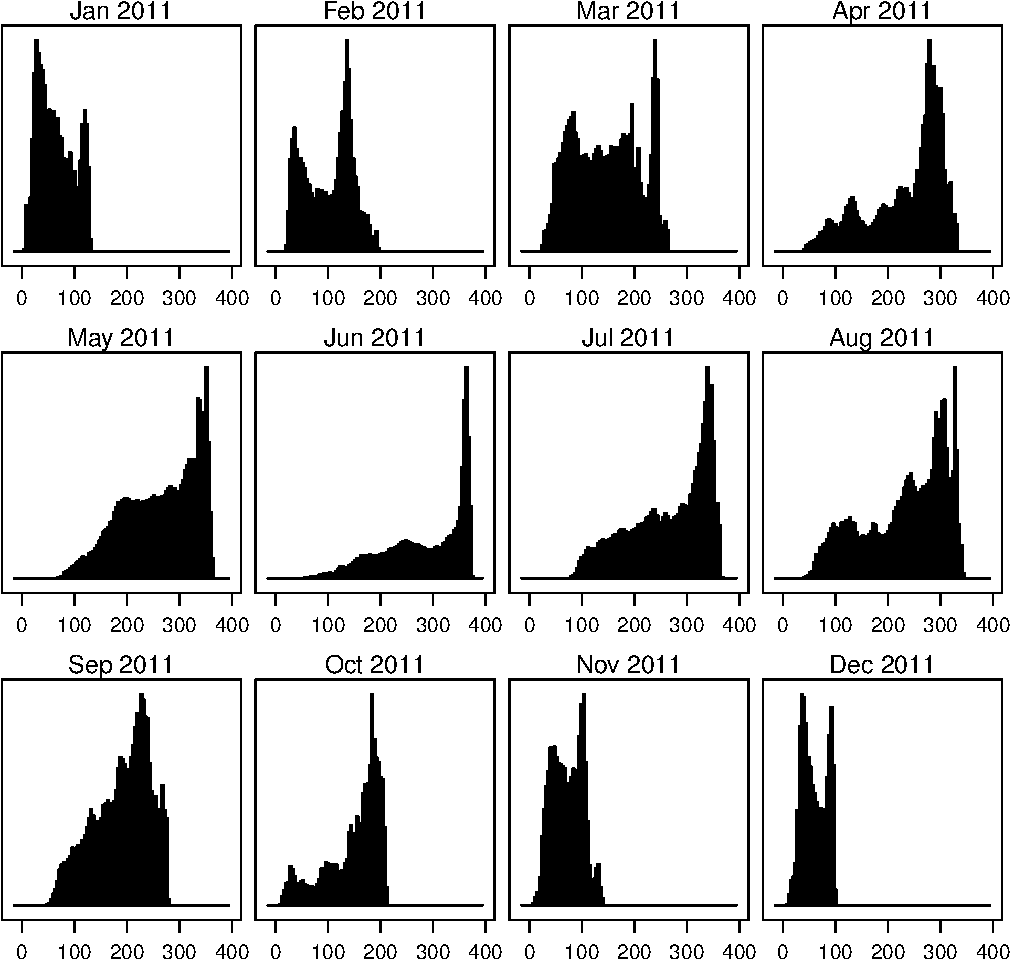
\includegraphics[width=.9\linewidth]{figs/SISdm_histogram.pdf}
\end{frame}

\begin{frame}[fragile,label=sec-4-8]{BWPlot}
 \lstset{language=R,label= ,caption= ,numbers=none}
\begin{lstlisting}
  bwplot(SISdm, FUN=as.yearmon)
\end{lstlisting}

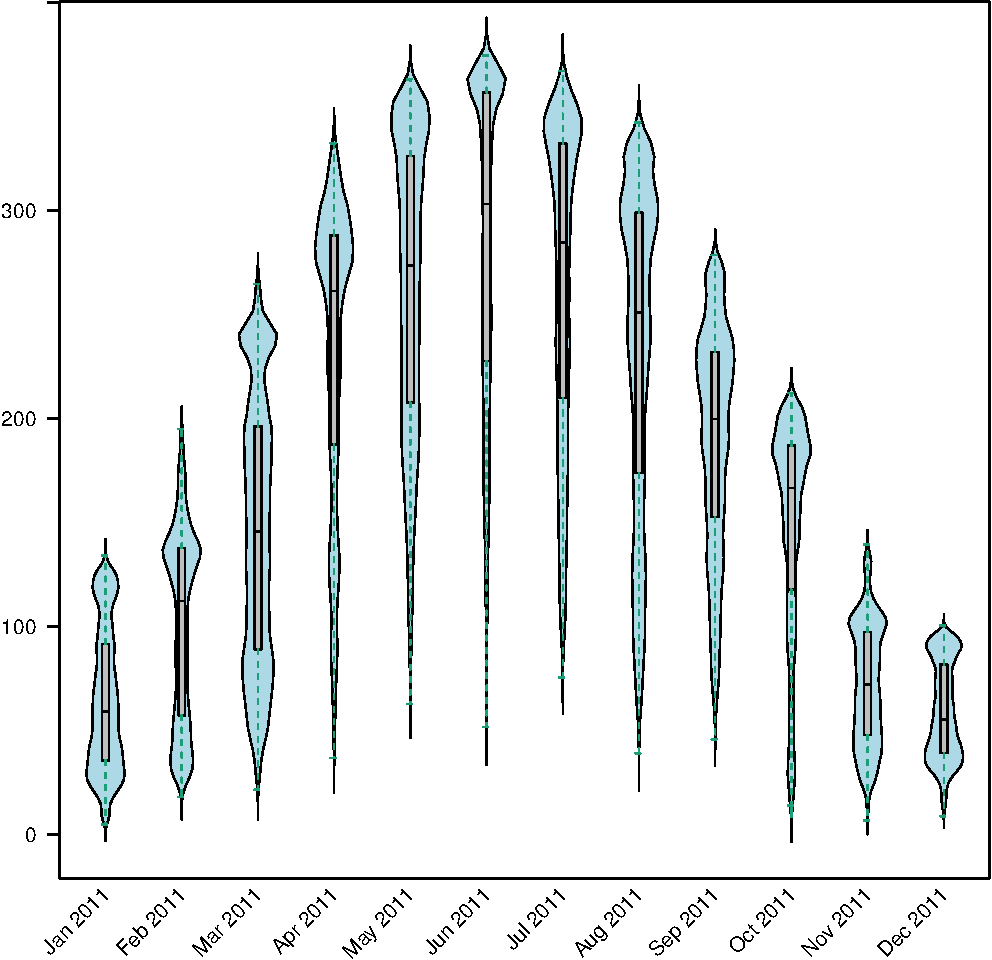
\includegraphics[width=.9\linewidth]{figs/SISdm_boxplot.pdf}
\end{frame}

\begin{frame}[fragile,label=sec-4-9]{Splom}
 \lstset{language=R,label= ,caption= ,numbers=none}
\begin{lstlisting}
  splom(SISmm, xlab='', plot.loess=TRUE)
\end{lstlisting}

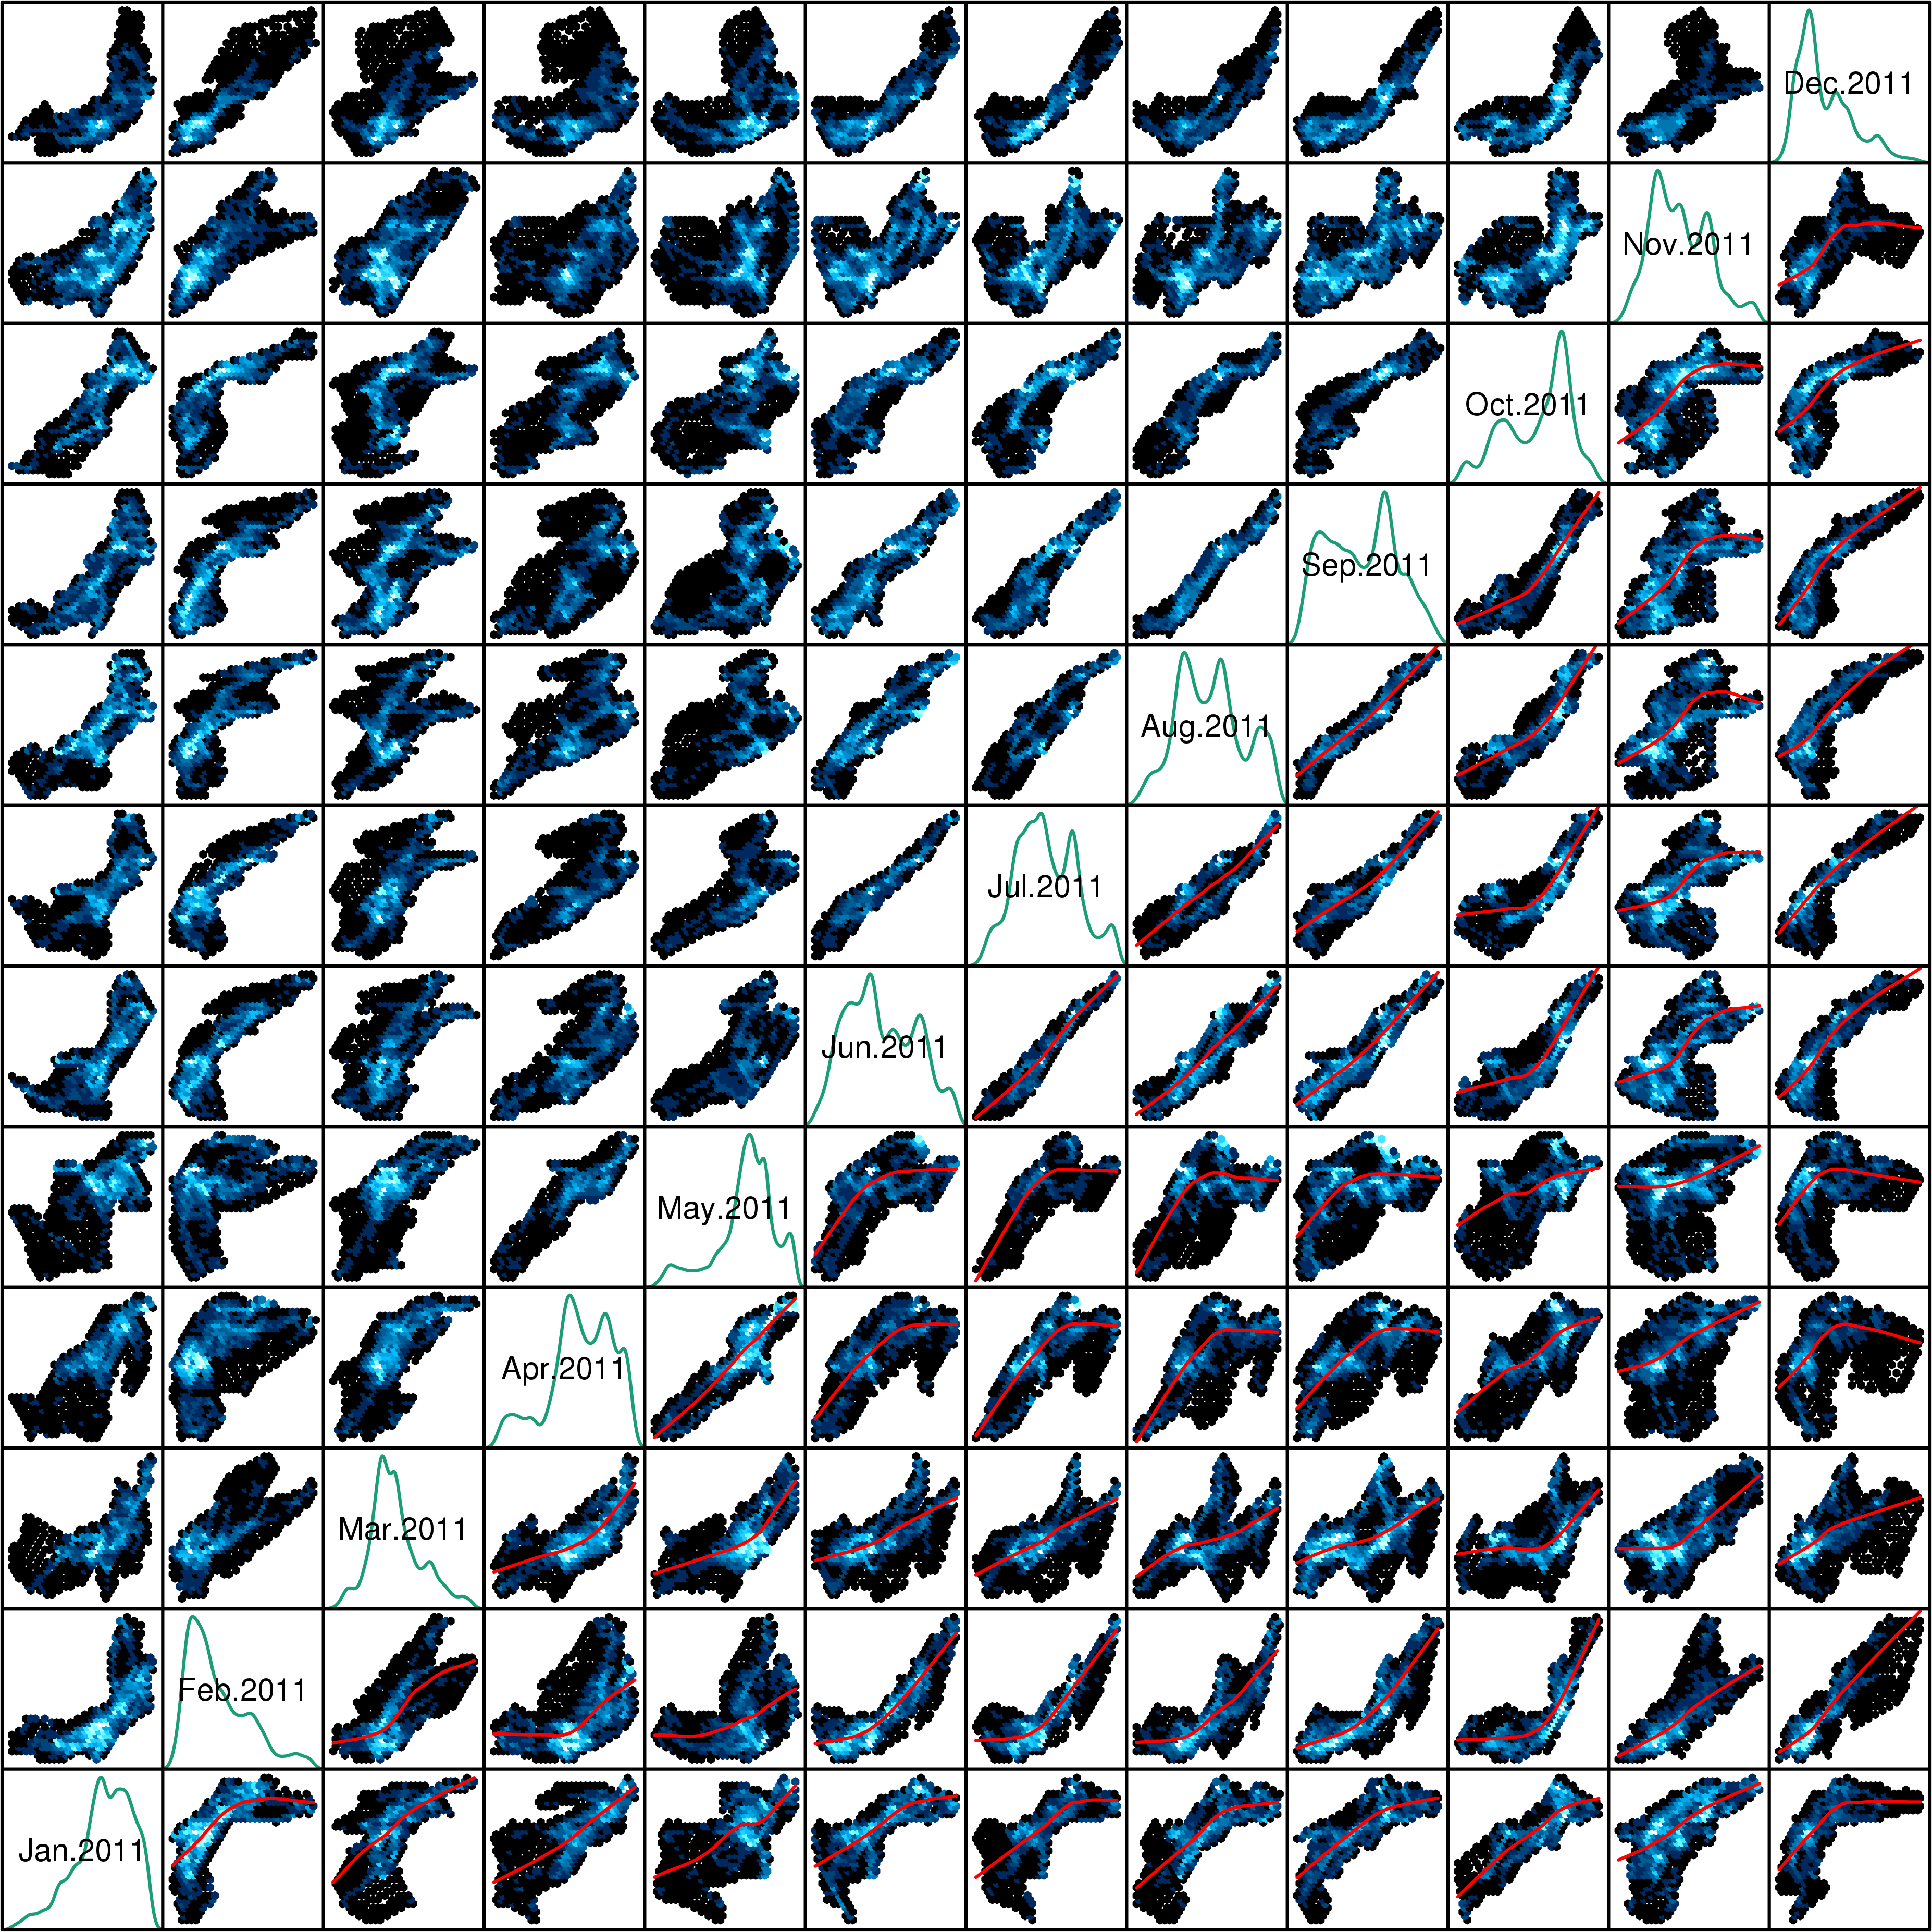
\includegraphics[width=.9\linewidth]{figs/SISmm_splom.png}
\end{frame}


\begin{frame}[label=sec-4-10]{Space-Time and Time Series Plots}
\end{frame}



\begin{frame}[fragile,label=sec-4-11]{Hovmoller}
 \lstset{language=R,label= ,caption= ,numbers=none}
\begin{lstlisting}
  hovmoller(SISdm, par.settings=BTCTheme())
\end{lstlisting}
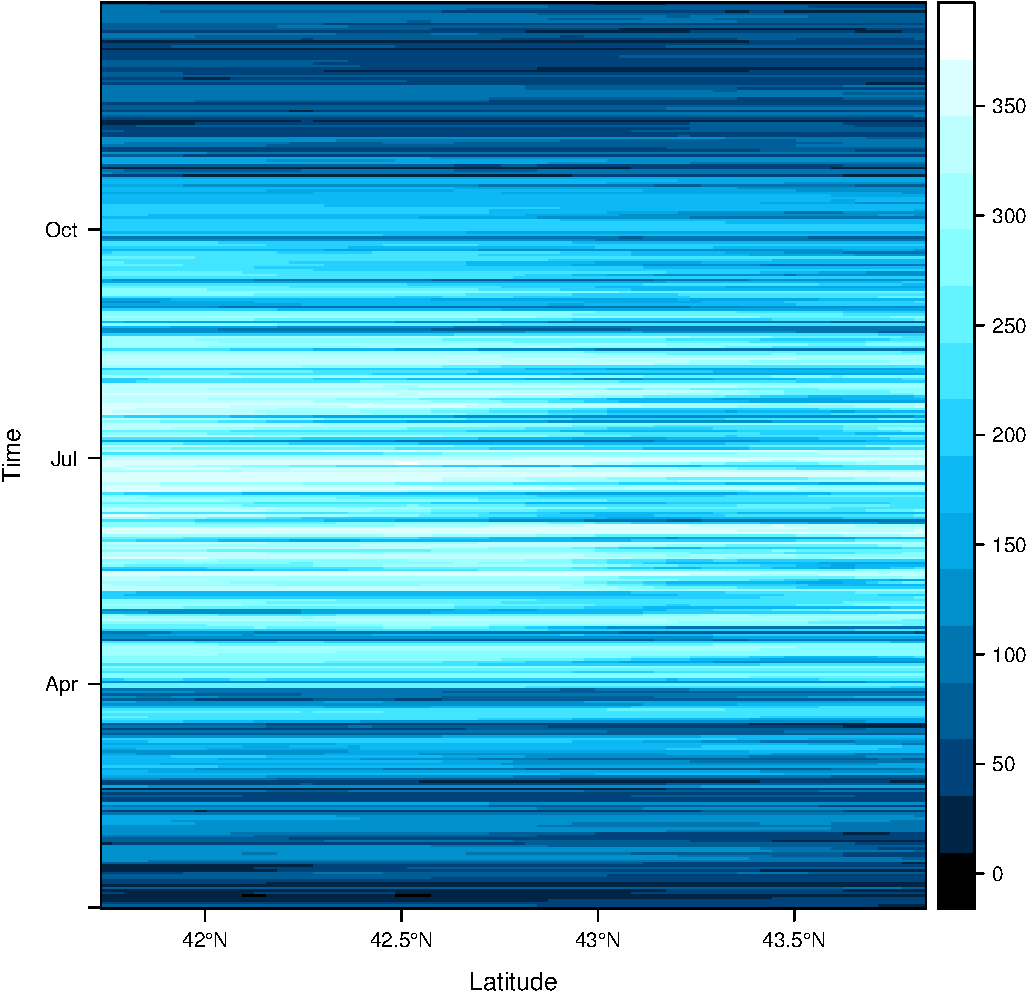
\includegraphics[width=.9\linewidth]{figs/SISdm_hovmoller_lat.pdf}
\end{frame}

\begin{frame}[fragile,label=sec-4-12]{xyplot}
 \lstset{language=R,label= ,caption= ,numbers=none}
\begin{lstlisting}
  xyplot(SISdm, digits=1, col='black', lwd=0.2, alpha=0.6)
\end{lstlisting}

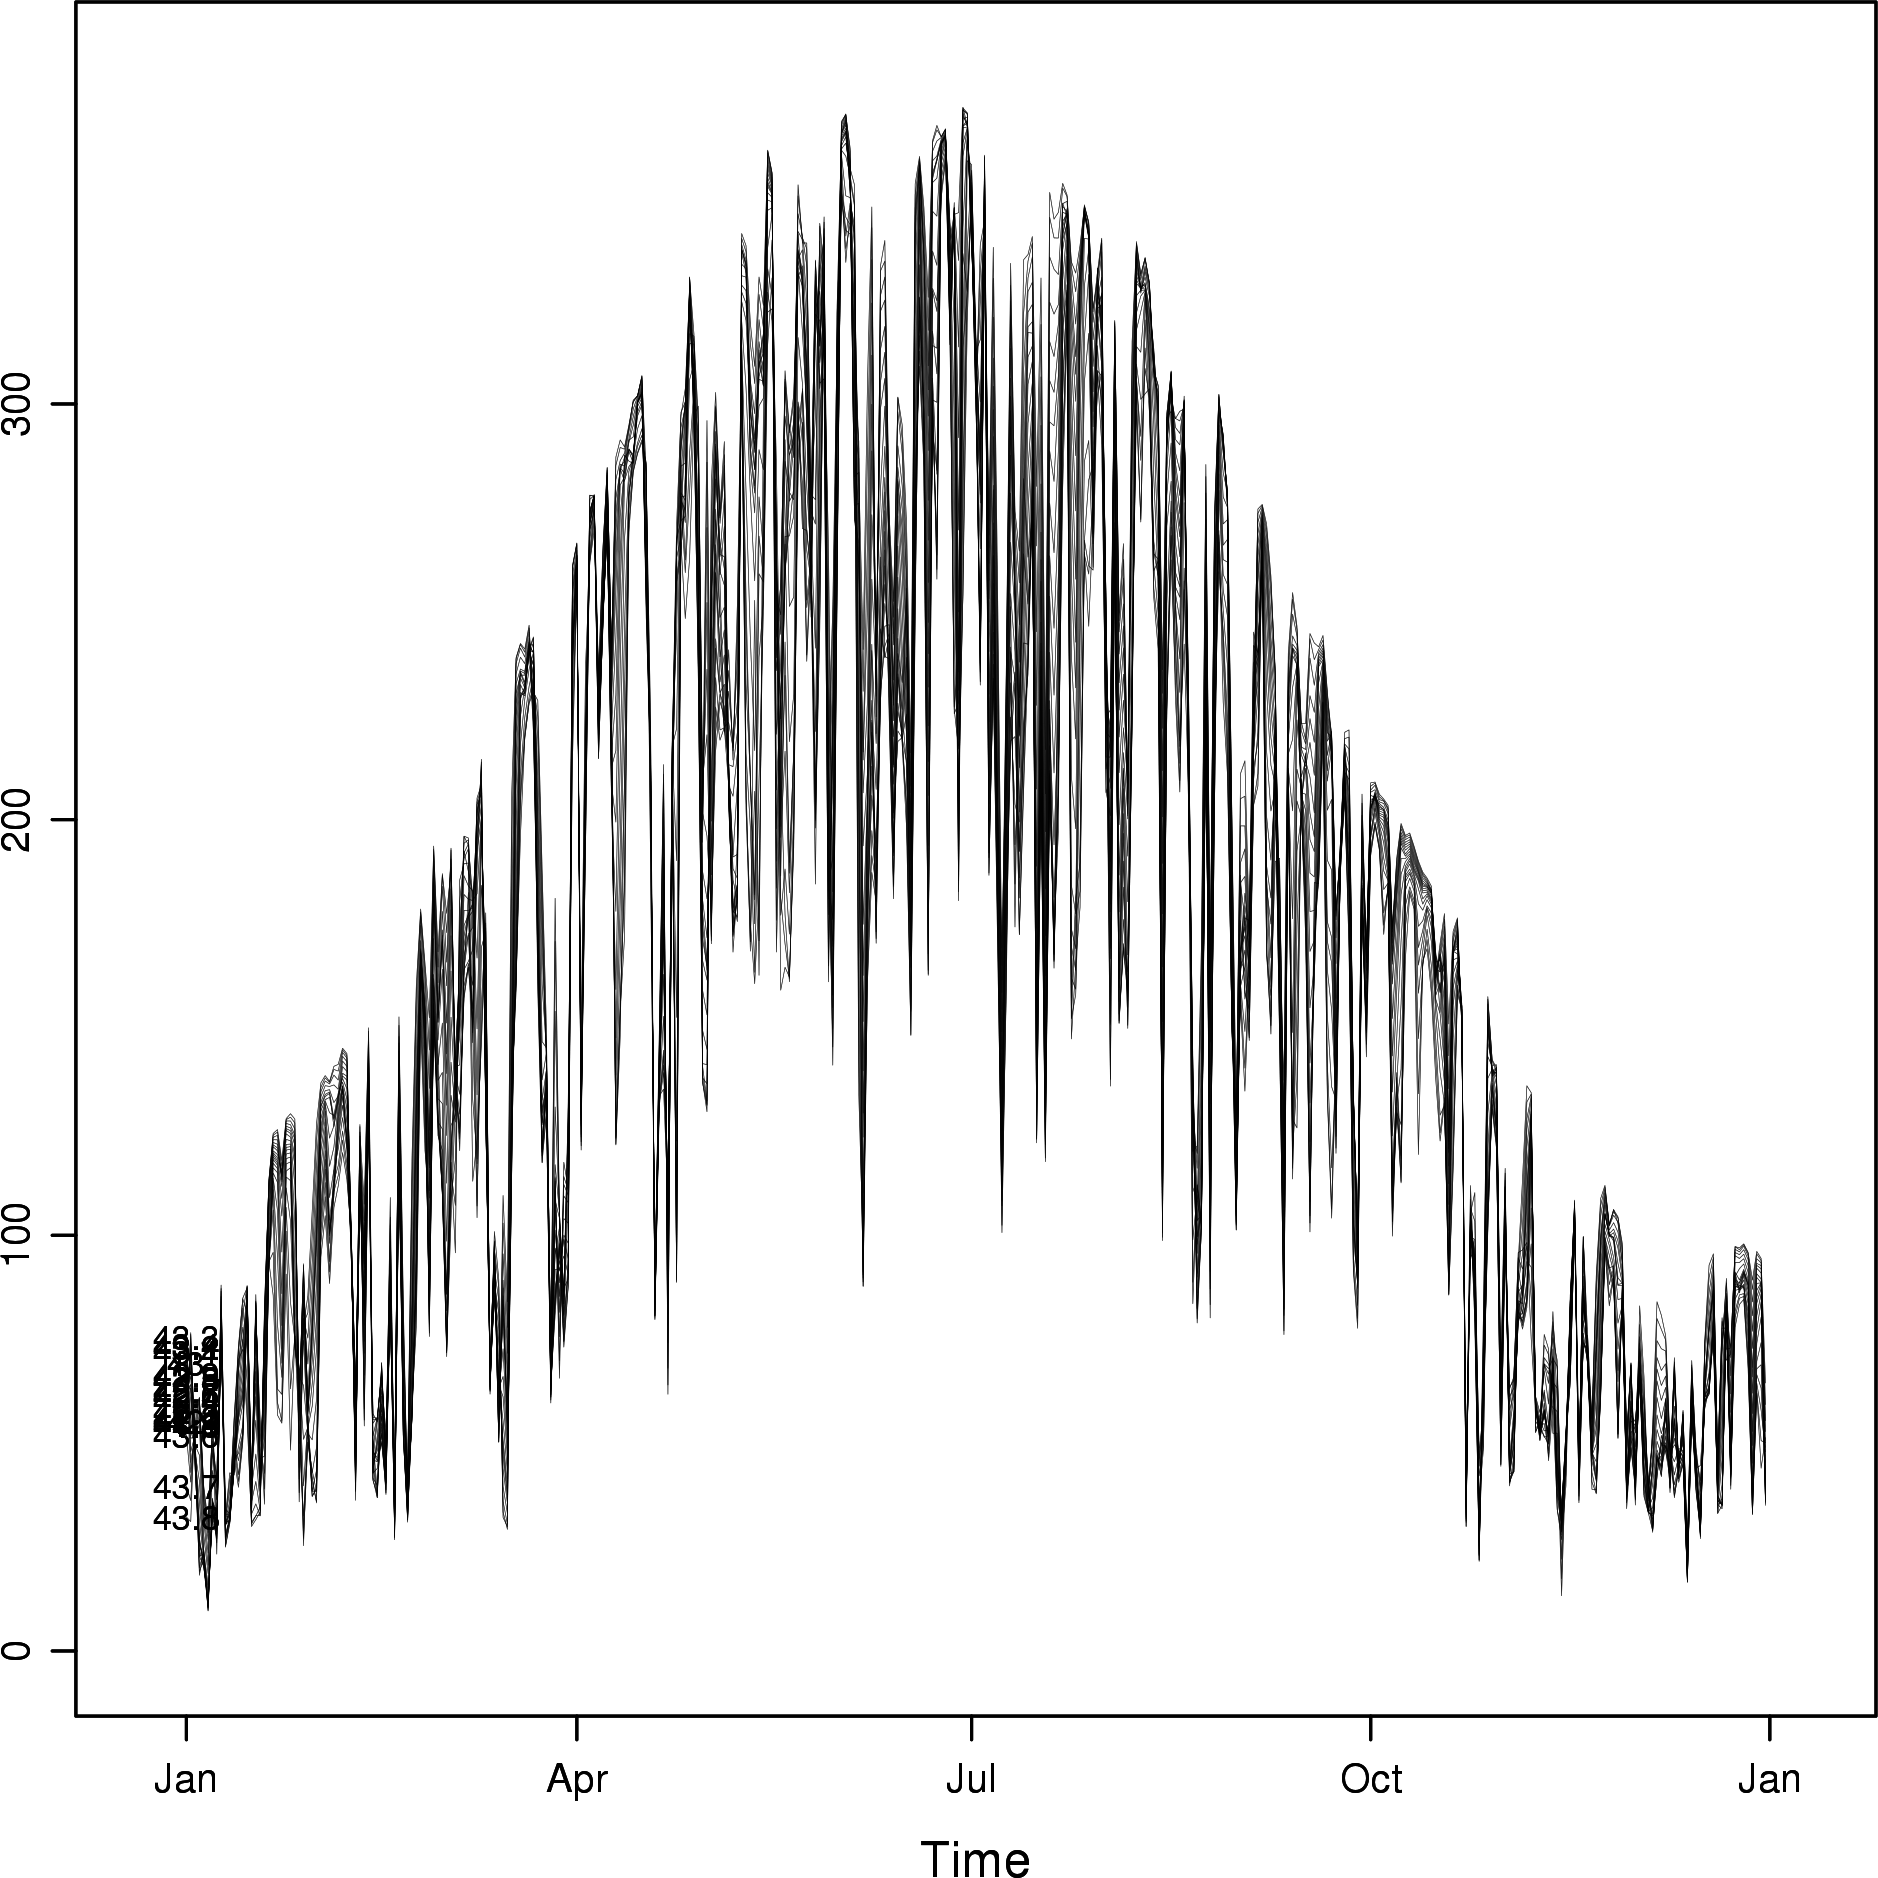
\includegraphics[width=.9\linewidth]{figs/SISmm_xyplot.png}
\end{frame}

\begin{frame}[fragile,label=sec-4-13]{Horizonplot}
 \lstset{language=R,label= ,caption= ,numbers=none}
\begin{lstlisting}
  horizonplot(SISdm, digits=1,
              col.regions=rev(brewer.pal(n=6, 'PuOr')),
              xlab='', ylab='Latitude')
\end{lstlisting}

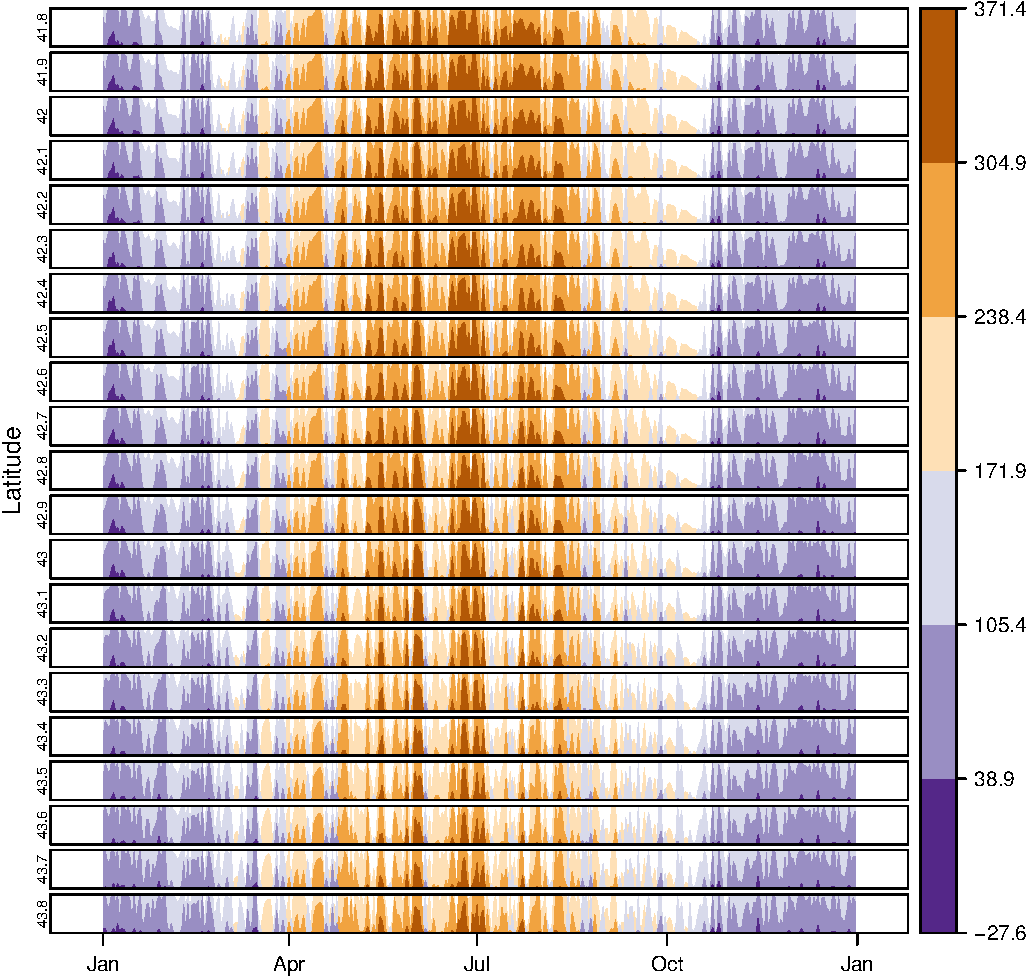
\includegraphics[width=.9\linewidth]{figs/SISdm_horizonplot.pdf}
\end{frame}


\begin{frame}[fragile,label=sec-4-14]{Animation}
 \lstset{language=R,label= ,caption= ,numbers=none}
\begin{lstlisting}
  cft <- brick('data/cft_20130417_0000.nc')
  ## use memory instead of file
  cft[] <- getValues(cft)
  ## set projection
  projLCC2d <- "+proj=lcc +lon_0=-14.1 +lat_0=34.823 +lat_1=43 +lat_2=43 +x_0=536402.3 +y_0=-18558.61 +units=km +ellps=WGS84"
  projection(cft) <- projLCC2d
  #set time index
  timeIndex <- seq(as.POSIXct('2013-04-17 01:00:00', tz='UTC'), length=96, by='hour')
  cft <- setZ(cft, timeIndex)
  names(cft) <- format(timeIndex, 'D%d_H%H')
\end{lstlisting}
\end{frame}


\begin{frame}[fragile,label=sec-4-15]{Spatial Context: Administrative Boundaries}
 \lstset{language=R,label= ,caption= ,numbers=none}
\begin{lstlisting}
  library(maptools)
  library(rgdal)
  library(maps)
  library(mapdata)
  
  
  projLL <- CRS('+proj=longlat +datum=WGS84 +ellps=WGS84 +towgs84=0,0,0')
  cftLL <- projectExtent(cft, projLL)
  cftExt <- as.vector(bbox(cftLL))
  boundaries <- map('worldHires',
                    xlim=cftExt[c(1,3)], ylim=cftExt[c(2,4)],
                    plot=FALSE)
  boundaries <- map2SpatialLines(boundaries, proj4string=projLL)
  boundaries <- spTransform(boundaries, CRS(projLCC2d))
\end{lstlisting}
\end{frame}


\begin{frame}[fragile,label=sec-4-16]{Producing the Frames and the Movie}
 \lstset{language=R,label= ,caption= ,numbers=none}
\begin{lstlisting}
  cloudTheme <- rasterTheme(region=brewer.pal(n=9, 'Blues'))
\end{lstlisting}

\lstset{language=R,label= ,caption= ,numbers=none}
\begin{lstlisting}
  tmp <- tempdir()
  trellis.device(png, file=paste0(tmp, '/Rplot%02d.png'),
                        res=300, width=1500, height=1500)
  levelplot(cft, layout=c(1, 1), par.settings=cloudTheme) +
      layer(sp.lines(boundaries, lwd=0.6))
  dev.off()
\end{lstlisting}
\end{frame}

\begin{frame}[fragile,label=sec-4-17]{ffmpeg}
 \lstset{language=R,label= ,caption= ,numbers=none}
\begin{lstlisting}
  old <- setwd(tmp)
  ## Create a movie with ffmpeg using 6 frames per second a bitrate of 300kbs
  movieCMD <- 'ffmpeg -r 6 -b 300k -i Rplot%02d.png output.mp4'
  system(movieCMD)
  file.remove(dir(pattern='Rplot'))
  file.copy('output.mp4', paste0(old, '/figs/cft.mp4'), overwrite=TRUE)
  setwd(old)
\end{lstlisting}

\href{http://vimeo.com/user18057623/cft}{Video}
\end{frame}

\begin{frame}[fragile,label=sec-4-18]{Static Image}
 \lstset{language=R,label= ,caption= ,numbers=none}
\begin{lstlisting}
  levelplot(cft, layers=25:48, layout=c(6, 4),
            par.settings=cloudTheme,
            names.attr=paste0(sprintf('%02d', 1:24), 'h'),
            panel=panel.levelplot.raster) +
      layer(sp.lines(boundaries, lwd=0.6))
\end{lstlisting}

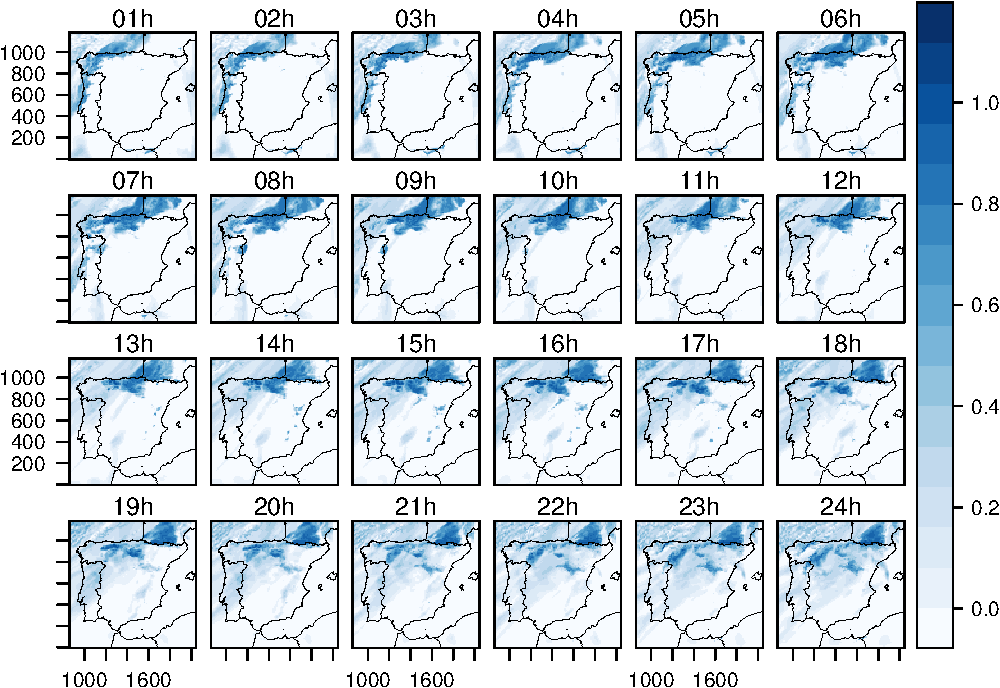
\includegraphics[width=.9\linewidth]{figs/cft.pdf}
\end{frame}


\section{Campos Vectoriales}
\label{sec-5}
\begin{frame}[label=sec-5-1]{Introducción}
\end{frame}

\begin{frame}[fragile,label=sec-5-2]{Data}
 \lstset{language=R,label= ,caption= ,numbers=none}
\begin{lstlisting}
  library(raster)
  library(rasterVis)
  
  wDir <- raster('data/wDir')/180*pi
  wSpeed <- raster('data/wSpeed')
  windField <- stack(wSpeed, wDir)
  names(windField) <- c('magnitude', 'direction')
\end{lstlisting}
\end{frame}


\begin{frame}[fragile,label=sec-5-3]{Vectorplot}
 \lstset{language=R,label= ,caption= ,numbers=none}
\begin{lstlisting}
  vectorplot(windField, isField=TRUE, par.settings=BTCTheme(),
             colorkey=FALSE, scales=list(draw=FALSE))
\end{lstlisting}


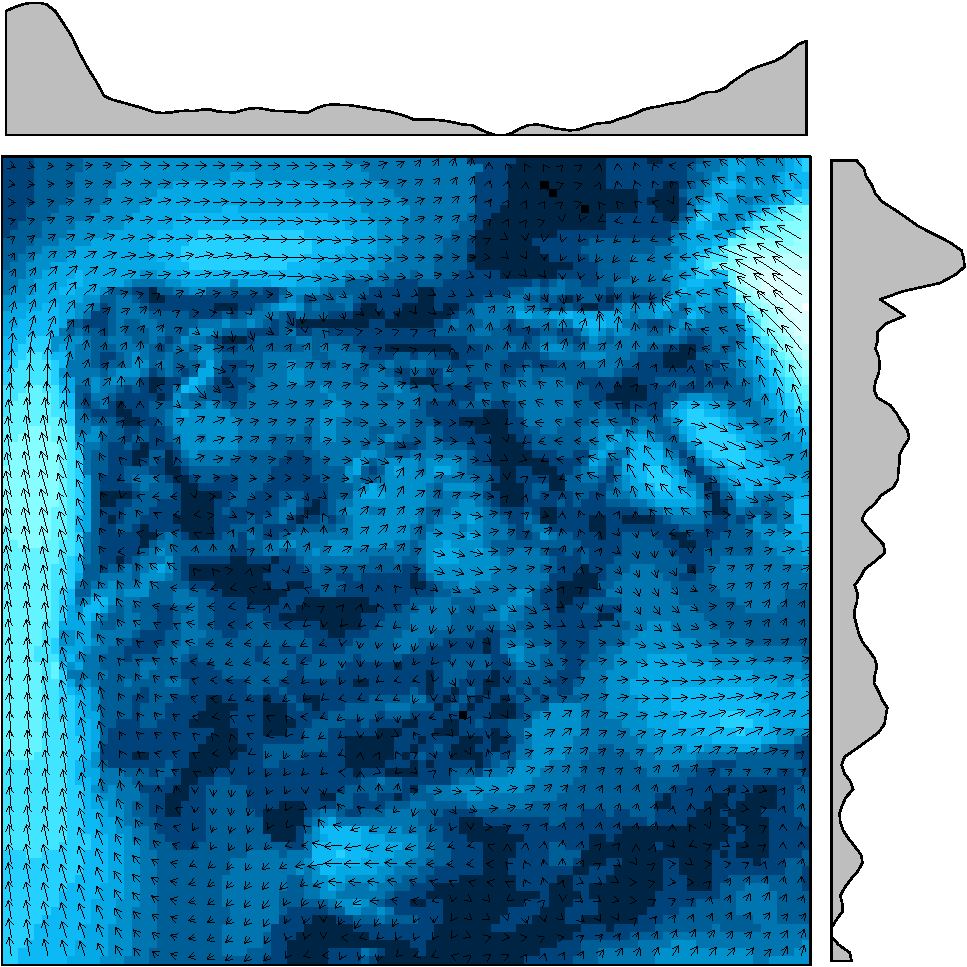
\includegraphics[width=.9\linewidth]{figs/vectorplot.pdf}
\end{frame}

\begin{frame}[label=sec-5-4]{streamlines}
\end{frame}

\begin{frame}[fragile,label=sec-5-5]{streamplot}
 \lstset{language=R,label= ,caption= ,numbers=none}
\begin{lstlisting}
  myTheme <- streamTheme(region=rev(brewer.pal(n=4, name='Greys')),
                                      symbol=BTC(n=9, beg=20))
  streamplot(windField, isField=TRUE,
             par.settings=myTheme,
             droplet=list(pc=12),
             streamlet=list(L=5, h=5),
             scales=list(draw=FALSE),
             panel=panel.levelplot.raster)
\end{lstlisting}
\end{frame}

\begin{frame}[label=sec-5-6]{}
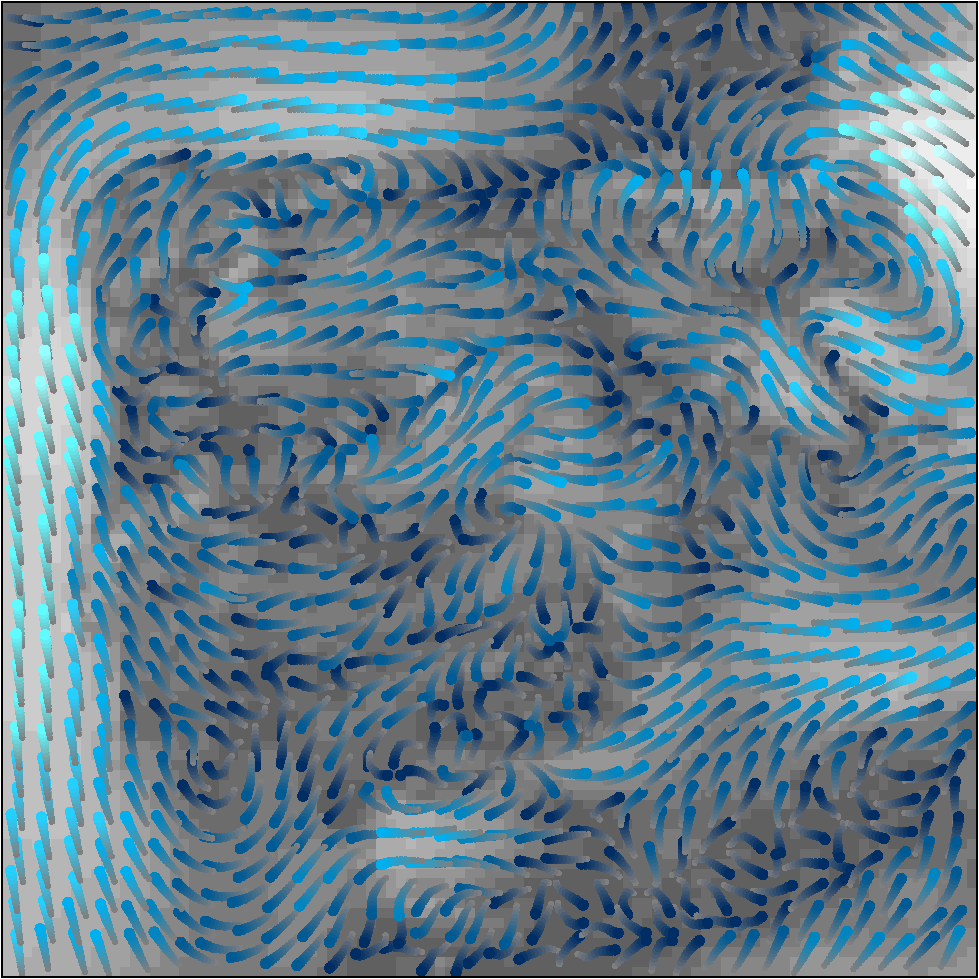
\includegraphics[width=.9\linewidth]{figs/streamplot.pdf}
\end{frame}

\begin{frame}[label=sec-5-7]{}

\end{frame}
% Emacs 24.3.1 (Org mode 8.2.7c)
\end{document}